\documentclass[12pt]{article}

\usepackage[a4paper, left = 1.5cm, right = 1.5cm, top = 1.5cm, bottom = 1.5cm]{geometry}

\usepackage{tikz}
\usetikzlibrary{positioning,fit,calc}
\tikzset{block/.style={draw,thick,text width=2cm,minimum height=1cm,align=center},
         line/.style={-latex}
}
\tikzstyle{arrow} = [thick,->,>=stealth]

\usepackage{amsmath}
\usepackage{amssymb}

\usepackage{hyperref}
\hypersetup {
	colorlinks=true,
	urlcolor=blue
}

\usepackage{pgfplots}
\usepackage{pgfplotstable}
\pgfplotsset{width=15cm,height=7cm,compat=newest}
\usepgfplotslibrary{fillbetween}

\usepackage{mathtools}

\usepackage{enumitem}

\usepackage{graphicx}
\usepackage{float}

\usepackage{diagbox}

\usepackage{karnaugh-map}

\usepackage[T1]{fontenc}

\usepackage{listings}
\usepackage{xcolor}
\usepackage{colortbl}

\usepackage{tabu}

\lstset{
	language = Python,
	backgroundcolor=\color{black!5}, % set backgroundcolor
	breaklines=true,
	postbreak=\mbox{\textcolor{red}{$\hookrightarrow$}\space},
}

\renewcommand{\baselinestretch}{1.5}

\renewcommand\thesection{\arabic{section}.}

\usepackage{tocloft}
\cftsetindents{section}{0em}{2em}
\cftsetindents{subsection}{0em}{2em}
\renewcommand\cfttoctitlefont{\hfill\Large\bfseries}
\renewcommand\cftaftertoctitle{\hfill\mbox{}}
\setcounter{tocdepth}{2}

\begin{document}
\begin{titlepage}
\centering
\vspace*{\fill}
\huge CS553: Cryptography\\
\LARGE Assignment 8: Solutions\\
\Large Rohit Das (11910230)\\\vspace{0.8cm}
\today
\vspace*{\fill}
\end{titlepage}

\begin{large}

\section{Authenticated Encryption Schemes}

\begin{enumerate}

\item \textbf{Nyberg and Rueppel Scheme}: It is an application of their signature scheme, which was the first discrete logarithm based scheme with message recovery.

\item \textbf{Keyak}: It is a scheme based on Keccak-p. It takes as input a secret and unique value (SUV), then some associated data (or metadata) that are authenticated but not encrypted and finally some plaintext.

\item \textbf{Wu and Hsu's Convertible Scheme}: A new authenticated encryption scheme with (t,n) shared verification based on discrete logarithms was proposed.

\item \textbf{Hwang's AE Scheme with Message Linkage}: To reduce costs for redundancies in message blocks, the scheme is divided into two parts, generation of signature and encryption phase, and recovery message and verification phase.

\item \textbf{Galois/Counter Mode (GCM) for Block Ciphers}: It is an authenticated encryption algorithm designed to provide both data authenticity and integrity.

\item \textbf{Carter-Wegman Counter Mode (CWC)}: It combines the use of CTR mode for encryption with an efficient polynomial Carter-Wegman MAC.

\item \textbf{Tiaoxin-346}: It is a nonce-based scheme, taking 4 inputs: Key K (128 bits), public nonce IV (128 bits), plaintext M (0 to $2 ^ {128}$ - 1 bits) and associated data AD (0 to $2 ^ {128}$ - 1 bits).

\item \textbf{Offset Codebook Mode (OCB)}: It is essentially a scheme to integrate a MAC into the operation of a block cipher.

\item \textbf{EAX}: It is an AEAD scheme designed to simultaneously provide both authenticity and privacy with a two-pass scheme.

\item \textbf{Sophie Germain Counter Mode (SGCM)}: Instead of the binary field $GF(2^{128})$, it used modular arithmetic in $GF(p)$, where $p$ is a safe prime $2^{128} + 12451$ with corresponding Sophie Germain prime $\dfrac{p-1}{2} = 2^{127} + 6225$. 

\end{enumerate}

\section{Hash: Mode-of-operation + collision}

\subsection{Pg. 315, Problem 11.3}

%\includegraphics[width = 0.45\linewidth]{./images/img1.jpg}
%\hspace{0.05\linewidth} \includegraphics[width = 0.45\linewidth]{./images/img2.jpg}\\
%
%\includegraphics[scale=•]{•} = 0.45\linewidth]{./images/img3.jpg}\\

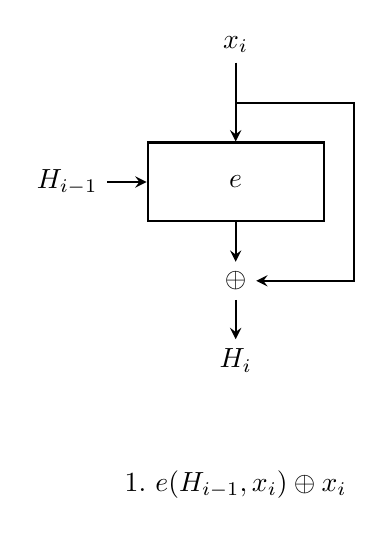
\begin{tikzpicture}

\node[block] (block) {$e$};
\node[draw=none,above=of block] (msg) {$x_i$};
\node[draw=none,left=0.5cm of block] (prevhash) {$H_{i - 1}$};
\node[draw=none,below=0.5cm of block] (xor) {$\oplus$};
\node[draw=none,below=0.5cm of xor] (hash) {$H_i$};
\node[draw=none,below=1cm of hash] (caption) {$1.$ $ e(H_{i-1},x_i)\oplus x_i$};
\draw[arrow] (msg)--(block);
\draw[arrow] (prevhash)--(block);
\draw[arrow] (block)--(xor);
\draw[arrow] (xor)--(hash);
\draw[arrow] (0,1)-|(1.5,0)|-(xor);

\end{tikzpicture}
\hspace{0.25\linewidth}
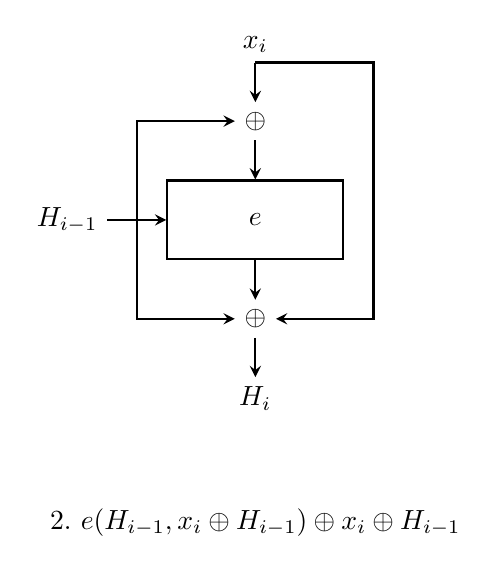
\begin{tikzpicture}

\node[block] (block) {$e$};
\node[draw=none,above=0.5cm of block] (xora) {$\oplus$};
\node[draw=none,above=0.5cm of xora] (msg) {$x_i$};
\node[draw=none,left=0.75cm of block] (prevhash) {$H_{i - 1}$};
\node[draw=none,below=0.5cm of block] (xor) {$\oplus$};
\node[draw=none,below=0.5cm of xor] (hash) {$H_i$};
\node[draw=none,below=1cm of hash] (caption) {$2.$ $ e(H_{i-1},x_i \oplus H_{i-1})\oplus x_i \oplus H_{i-1}$};
\draw[arrow] (msg)--(xora);
\draw[arrow] (xora)--(block);
\draw[arrow] (prevhash)--(block);
\draw[arrow] (block)--(xor);
\draw[arrow] (xor)--(hash);
\draw[arrow] (0,2)-|(1.5,0)|-(xor);
\draw[arrow] (-1.5,0)|-(xora);
\draw[arrow] (-1.5,0)|-(xor);

\end{tikzpicture}

\vspace{0.75cm}
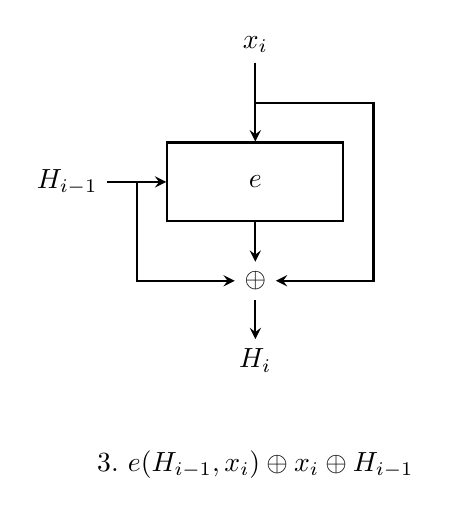
\begin{tikzpicture}

\node[block] (block) {$e$};
\node[draw=none,above=of block] (msg) {$x_i$};
\node[draw=none,left=0.75cm of block] (prevhash) {$H_{i - 1}$};
\node[draw=none,below=0.5cm of block] (xor) {$\oplus$};
\node[draw=none,below=0.5cm of xor] (hash) {$H_i$};
\node[draw=none,below=0.75cm of hash] (caption) {$3.$ $ e(H_{i-1},x_i)\oplus x_i \oplus H_{i-1}$};
\draw[arrow] (msg)--(block);
\draw[arrow] (prevhash)--(block);
\draw[arrow] (block)--(xor);
\draw[arrow] (xor)--(hash);
\draw[arrow] (0,1)-|(1.5,0)|-(xor);
\draw[arrow] (-1.5,0)|-(xor);

\end{tikzpicture}
\hspace{0.15\linewidth}
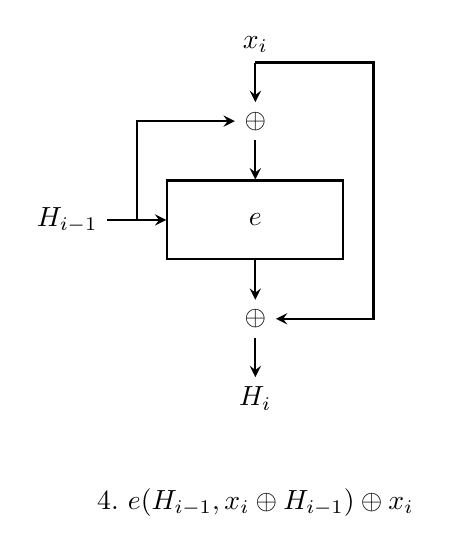
\begin{tikzpicture}

\node[block] (block) {$e$};
\node[draw=none,above=0.5cm of block] (xora) {$\oplus$};
\node[draw=none,above=0.5cm of xora] (msg) {$x_i$};\node[draw=none,left=0.75cm of block] (prevhash) {$H_{i - 1}$};
\node[draw=none,below=0.5cm of block] (xor) {$\oplus$};
\node[draw=none,below=0.5cm of xor] (hash) {$H_i$};
\node[draw=none,below=0.75cm of hash] (caption) {$4.$ $ e(H_{i-1},x_i \oplus H_{i-1})\oplus x_i$};
\draw[arrow] (msg)--(xora);
\draw[arrow] (xora)--(block);
\draw[arrow] (prevhash)--(block);
\draw[arrow] (block)--(xor);
\draw[arrow] (xor)--(hash);
\draw[arrow] (-1.5,0)|-(xora);
\draw[arrow] (0,2)-|(1.5,0)|-(xor);

\end{tikzpicture}

\vspace{0.75cm}
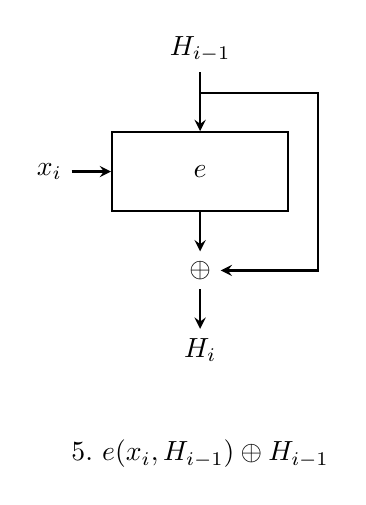
\begin{tikzpicture}

\node[block] (block) {$e$};
\node[draw=none,left=0.5cm of block] (msg) {$x_i$};
\node[draw=none,above=0.75cm of block] (prevhash) {$H_{i - 1}$};
\node[draw=none,below=0.5cm of block] (xor) {$\oplus$};
\node[draw=none,below=0.5cm of xor] (hash) {$H_i$};
\node[draw=none,below=0.75cm of hash] (caption) {$5.$ $ e(x_i,H_{i-1})\oplus H_{i-1}$};
\draw[arrow] (msg)--(block);
\draw[arrow] (prevhash)--(block);
\draw[arrow] (block)--(xor);
\draw[arrow] (xor)--(hash);
\draw[arrow] (0,1)-|(1.5,0)|-(xor);

\end{tikzpicture}
\hspace{0.25\linewidth}
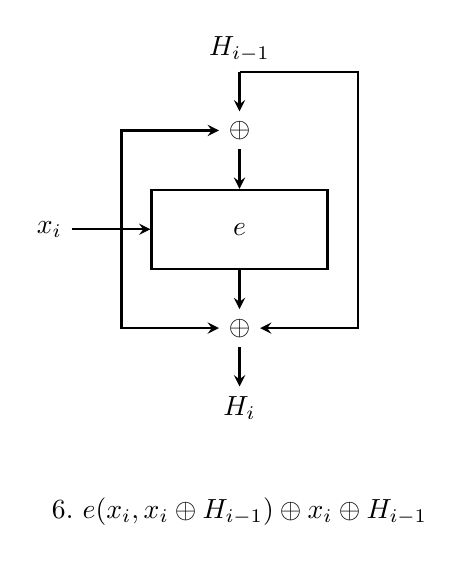
\begin{tikzpicture}

\node[block] (block) {$e$};
\node[draw=none,left=of block] (msg) {$x_i$};
\node[draw=none,above=0.5cm of block] (xora) {$\oplus$};
\node[draw=none,above=0.5cm of xora] (prevhash) {$H_{i - 1}$};
\node[draw=none,below=0.5cm of block] (xor) {$\oplus$};
\node[draw=none,below=0.5cm of xor] (hash) {$H_i$};
\node[draw=none,below=0.75cm of hash] (caption) {$6.$ $ e(x_i,x_i \oplus H_{i-1})\oplus x_i \oplus H_{i-1}$};
\draw[arrow] (prevhash)--(xora);
\draw[arrow] (xora)--(block);
\draw[arrow] (msg)--(block);
\draw[arrow] (block)--(xor);
\draw[arrow] (xor)--(hash);
\draw[arrow] (0,2)-|(1.5,0)|-(xor);
\draw[arrow] (-1.5,0)|-(xora);
\draw[arrow] (-1.5,0)|-(xor);

\end{tikzpicture}

\vspace{0.75cm}
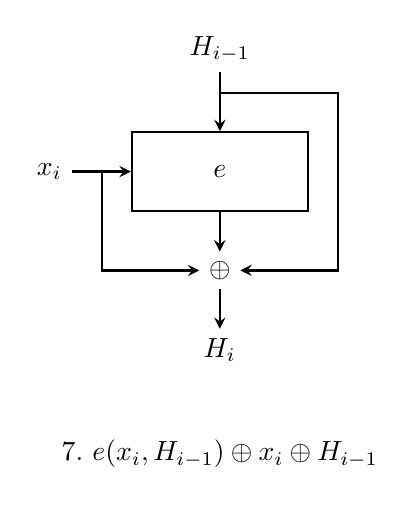
\begin{tikzpicture}

\node[block] (block) {$e$};
\node[draw=none,left=0.75cm of block] (msg) {$x_i$};
\node[draw=none,above=0.75cm of block] (prevhash) {$H_{i - 1}$};
\node[draw=none,below=0.5cm of block] (xor) {$\oplus$};
\node[draw=none,below=0.5cm of xor] (hash) {$H_i$};
\node[draw=none,below=0.75cm of hash] (caption) {$7.$ $ e(x_i,H_{i-1})\oplus x_i \oplus H_{i-1}$};
\draw[arrow] (msg)--(block);
\draw[arrow] (prevhash)--(block);
\draw[arrow] (block)--(xor);
\draw[arrow] (xor)--(hash);
\draw[arrow] (0,1)-|(1.5,0)|-(xor);
\draw[arrow] (-1.5,0)|-(xor);

\end{tikzpicture}
\hspace{0.20\linewidth}
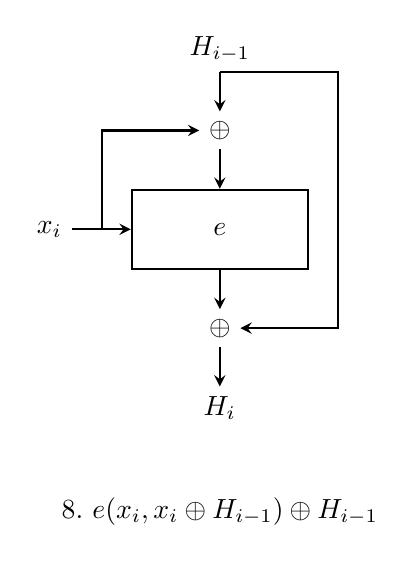
\begin{tikzpicture}

\node[block] (block) {$e$};
\node[draw=none,above=0.5cm of block] (xora) {$\oplus$};
\node[draw=none,left=0.75cm of block] (msg) {$x_i$};
\node[draw=none,above=0.5cm of xora] (prevhash) {$H_{i - 1}$};
\node[draw=none,below=0.5cm of block] (xor) {$\oplus$};
\node[draw=none,below=0.5cm of xor] (hash) {$H_i$};
\node[draw=none,below=0.75cm of hash] (caption) {$8.$ $ e(x_i,x_i \oplus H_{i-1})\oplus H_{i-1}$};
\draw[arrow] (prevhash)--(xora);
\draw[arrow] (xora)--(block);
\draw[arrow] (msg)--(block);
\draw[arrow] (block)--(xor);
\draw[arrow] (xor)--(hash);
\draw[arrow] (0,2)-|(1.5,0)|-(xor);
\draw[arrow] (-1.5,0)|-(xora);

\end{tikzpicture}

\vspace{0.75cm}
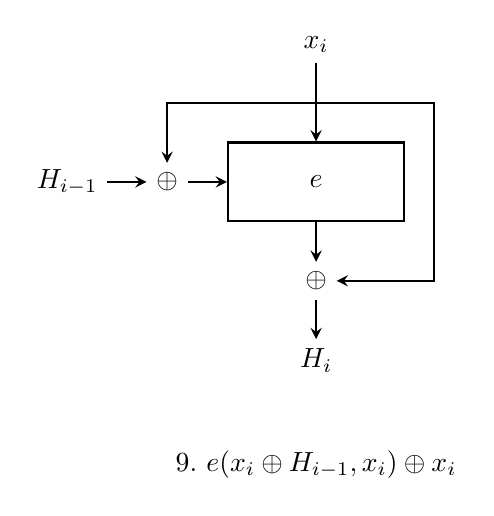
\begin{tikzpicture}

\node[block] (block) {$e$};
\node[draw=none,left=0.5cm of block] (xora) {$\oplus$};
\node[draw=none,above=of block] (msg) {$x_i$};
\node[draw=none,left=0.5cm of xora] (prevhash) {$H_{i - 1}$};
\node[draw=none,below=0.5cm of block] (xor) {$\oplus$};
\node[draw=none,below=0.5cm of xor] (hash) {$H_i$};
\node[draw=none,below=0.75cm of hash] (caption) {$9.$ $ e(x_i \oplus H_{i-1},x_i)\oplus x_i$};
\draw[arrow] (msg)--(block);
\draw[arrow] (prevhash)--(xora);
\draw[arrow] (xora)--(block);
\draw[arrow] (block)--(xor);
\draw[arrow] (xor)--(hash);
\draw[arrow] (0,1)-|(1.5,0)|-(xor);
\draw[arrow] (0,1)-|(xora);

\end{tikzpicture}
\hspace{0.10\linewidth}
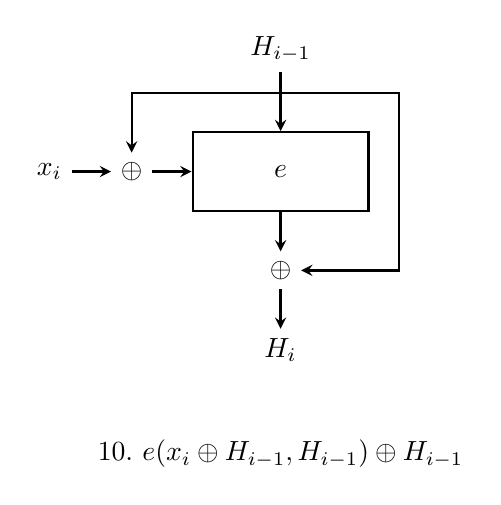
\begin{tikzpicture}

\node[block] (block) {$e$};
\node[draw=none,left=0.5cm of block] (xora) {$\oplus$};
\node[draw=none,left=0.5cm of xora] (msg) {$x_i$};
\node[draw=none,above=0.75cm of block] (prevhash) {$H_{i - 1}$};
\node[draw=none,below=0.5cm of block] (xor) {$\oplus$};
\node[draw=none,below=0.5cm of xor] (hash) {$H_i$};
\node[draw=none,below=0.75cm of hash] (caption) {$10.$ $ e(x_i \oplus H_{i-1},H_{i-1})\oplus H_{i-1}$};
\draw[arrow] (msg)--(xora);
\draw[arrow] (xora)--(block);
\draw[arrow] (prevhash)--(block);
\draw[arrow] (block)--(xor);
\draw[arrow] (xor)--(hash);
\draw[arrow] (0,1)-|(1.5,0)|-(xor);
\draw[arrow] (0,1)-|(xora);

\end{tikzpicture}

\vspace{0.75cm}
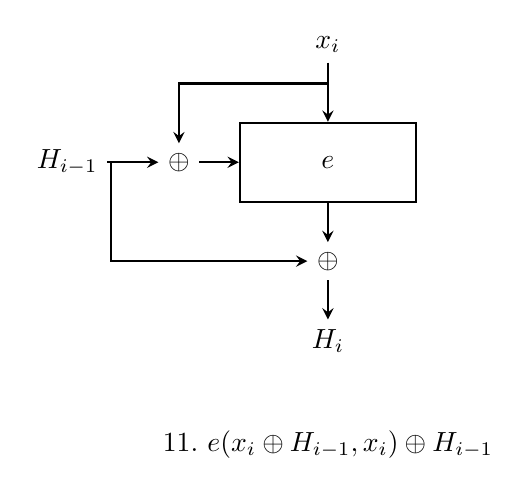
\begin{tikzpicture}

\node[block] (block) {$e$};
\node[draw=none,left=0.5cm of block] (xora) {$\oplus$};
\node[draw=none,above=0.75cm of block] (msg) {$x_i$};
\node[draw=none,left=0.65cm of xora] (prevhash) {$H_{i - 1}$};
\node[draw=none,below=0.5cm of block] (xor) {$\oplus$};
\node[draw=none,below=0.5cm of xor] (hash) {$H_i$};
\node[draw=none,below=0.75cm of hash] (caption) {$11.$ $ e(x_i \oplus H_{i-1},x_i)\oplus H_{i-1}$};
\draw[arrow] (prevhash)--(xora);
\draw[arrow] (xora)--(block);
\draw[arrow] (msg)--(block);
\draw[arrow] (block)--(xor);
\draw[arrow] (xor)--(hash);
\draw[arrow] (0,1)-|(xora);
\draw[arrow] (-2.75,0)|-(xor);

\end{tikzpicture}
\hspace{0.075\linewidth}
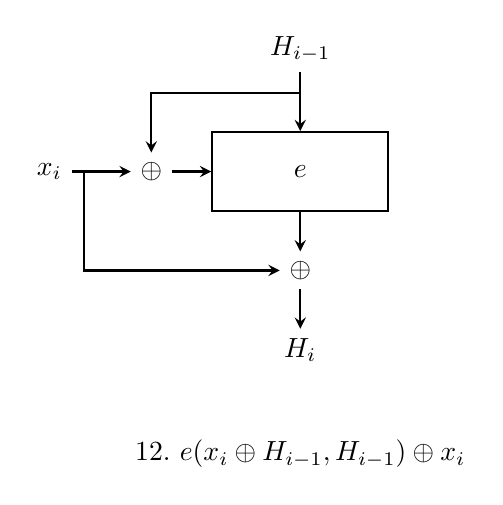
\begin{tikzpicture}

\node[block] (block) {$e$};
\node[draw=none,left=0.5cm of block] (xora) {$\oplus$};
\node[draw=none,left=0.75cm of xora] (msg) {$x_i$};
\node[draw=none,above=0.75cm of block] (prevhash) {$H_{i - 1}$};
\node[draw=none,below=0.5cm of block] (xor) {$\oplus$};
\node[draw=none,below=0.5cm of xor] (hash) {$H_i$};
\node[draw=none,below=0.75cm of hash] (caption) {$12.$ $ e(x_i \oplus H_{i-1},H_{i-1})\oplus x_i$};
\draw[arrow] (msg)--(xora);
\draw[arrow] (xora)--(block);
\draw[arrow] (prevhash)--(block);
\draw[arrow] (block)--(xor);
\draw[arrow] (xor)--(hash);
\draw[arrow] (0,1)-|(xora);
\draw[arrow] (-2.75,0)|-(xor);

\end{tikzpicture}

\newpage
\subsection{Pg. 316, Problem 11.8}

Python Code (Python3): hashing.py
\lstinputlisting[language=Python,showstringspaces=false]{./python_code/hashing.py}
Output: The hash function can be broken by choosing such characters whose bits will XOR out to be the XOR of bits of the target character. E.g., "CRYPTO" hashes to 110011, which is the same for "FINALE". The crucial property missing in this hash function is the second-preimage resistance,i.e., given a message $M_1$, we are easily able to find another message $M_2$ hashing to the same value as $M_1$.
\begin{lstlisting}
String: CRYPTO
Binary: 01000011 01010010 01011001 01010000 01010100 01001111 
Hash: 110011
String: FINALE
Binary: 01000110 01001001 01001110 01000001 01001100 01000101 
Hash: 110011
\end{lstlisting}

\section{Partial Collision: md5}

The list of $2^{16}$ pairs of strings and their corresponding hashes was generated 4 times to find collision in the first and last 16 bits of the hash. Hence, the total number of trials stands at $2^{18}$ = 262144. The strings have been generated randomly and hence may not form meaningful sentences.\\
Python Code (Python3): md5hash.py
\lstinputlisting[language=Python,showstringspaces=false]{./python_code/md5hash.py}
Output:\\
\includegraphics[width=\linewidth]{./images/img3.png}

\section{SSL Certificates: X509 Format}

\subsection{About X.509}

X.509 is a standard defining the format of public key certificates. An X.509 certificate contains a public key and an identity, and is either signed by a certificate authority, or self-signed. 

In this system, an organization that wants a signed certificate requests one via a certificate signing request (CSR). To do this, it first generates a key pair, keeping the private key secret and using it to sign the CSR. This contains information identifying the applicant and the applicant's public key that is used to verify the signature of the CSR - and the Distinguished Name (DN) that the certificate is for. The CSR may be accompanied by other credentials or proofs of identity required by the certificate authority.

There are several commonly used filename extensions for X.509 certificates. Some of these extensions are also used for other data such as private keys.

\begin{itemize}

\item .pem - (Privacy-enhanced Electronic Mail) Base64 encoded DER certificate, enclosed between "-----BEGIN CERTIFICATE-----" and "-----END CERTIFICATE-----"

\item .cer, .crt, .der - usually in binary DER form, but Base64-encoded certificates are common too (see .pem above)

\item .p7b, .p7c - PKCS\# 7 SignedData structure without data, just certificate(s) or CRL(s)

\item .p12 - PKCS\# 12, may contain certificate(s) (public) and private keys (password protected)

\item .pfx - PFX, predecessor of PKCS\# 12 (usually contains data in PKCS\# 12 format, e.g., with PFX files generated in IIS)

\end{itemize}

\subsection{SSL verification}

Command to download SSL certificate from www.facebook.com:
\begin{lstlisting}
openssl s_client -connect www.facebook.com:443 2>/dev/null </dev/null |  openssl x509 -outform PEM > fb_cert.pem
\end{lstlisting}
\vspace{0.25cm}
Command to verify SHA-1 fingerprint of above certificate:
\begin{lstlisting}
openssl x509 -noout -in fb_cert.pem -fingerprint -sha1
\end{lstlisting}
\vspace{0.25cm}
Generated Fingerprint:\\
SHA1 Fingerprint=A4:27:D4:9C:21:BD:B6:E4:52:B3:F8:D6:DE:25:79:3A:8C:0E:45:2A\\

\begin{figure}[H]
\centering
\includegraphics[width = 0.70\linewidth]{./images/img2.png}
\caption{Screenshot from Google Chrome browser of actual fingerprint}
\end{figure}

\section{MAC: Timing Attacks}

Python Code (Python3): timing$\_$attack.py
\lstinputlisting[language=Python,showstringspaces=false]{./python_code/timing_attack.py}
Output:

\begin{figure}[H]
\centering
\includegraphics[width = 0.62\linewidth]{./images/img1.png}

\caption{As evident from the screenshot, for compare$\_$mac(), comparing identical strings takes more time than for different strings. However, it is not so distinguishable in const$\_$compare$\_$mac().}

\end{figure}

\end{large}

\end{document}